\documentclass[a4]{article}

\usepackage[utf8]{inputenc}
\usepackage{graphicx}
\graphicspath{{./figs/}}

\title{Plasma line HOWTO}
\author{Carl-Fredrik Enell}

\begin{document}
\pagestyle{empty}

\maketitle{}
\thispagestyle{empty}

\section{Introduction}
\label{sec:introduction}

Incoherent scatter radars including EISCAT sometimes record enhanced
plasma lines. When this is the case, these provide a direct measure of
electron density independent of absolute power calibration.  Thus,
power calibration of an ISR can be performed by comparing plasma line
frequencies to peak electron densities from the ion line analysis.  At
EISCAT this is necessary in particular during the long winter season
when snow may accumulate in the antennas. This is especially important
for the fixed 42 m antenna of the Svalbard radar.

This document is a brief summary of the plasma line calibration procedure.



\section{Integrate plasma line data}
\label{sec:integr-plasma-line}

Before anything can be done, received plasma line data should be
integrated for a suitable period e.g. 60 seconds. The procedure is
different for different experiments and receivers.


\subsection{Separate plasma and ion line lag profiles in same files (mainland beata)}
\label{sec:plasma-ion-lines}

The plasma line integration procedure is similar to a normal GUISDAP
run. Select data path and interval and keep the settings the same as
for the normal analysis (like integration time and / or the necessary antenna scan parameters),
except that the following special parameter
should be typed into the Special window:

\begin{verbatim}
analysis_plasmaline=1;
\end{verbatim}
?? Ingemar should one also select site P ??

With this setting, GUISDAP will save integrated plasma line data.
When using the AUTO setting, the output directories will be named like
normal analysis directories but with site codes like \texttt{@Tp} (for UHF data).


\subsection{One ion-plasma line window (mainland bella)}

There are long lag experiments (at least bella) intended to contain ion and plasma lines in one spectral window. 

?? Ingemar, how does this work ??


\subsection{Separate plasma line data (ESR)}
\label{sec:separate-plasma-line}

ESR has separate plasma line receiver channels, so the plasma line
data will be stored in their own data directories. These have the
antenna name code \texttt{@32p}. When such a data directory is selected, GUISDAP will automatically go to the plasma line integration mode, so no special settings should be necessary. Just remember to select where the output should go.
If site P is chosen, however, the AUTO directories will get names ending in (integration time)@P, which makes it easier to separate directories, so this setting is recommended.

(?? If this does not work then select P and analysis\_plasmaline manually ??)

?? are there different cases e.g. also experiments not using the
separate plasma receiver but still containing plasmalines ??

For dual-antenna experiments like folke, the files will contain data from both antennas. The calibration routine will ask which antenna to use when given such input.


\clearpage{}

\section{Run plasma line calibration}
\label{sec:run-plasma-line}

The plasma calibration routine is \texttt{calib\_pl\_ne} and should be
called from a GUISDAP prompt.  The minimum required argument is the
path to the integrated plasma line data. If only the path is given,
the program will first show an overview plot of spectrograms for a
number of range intervals. It will then ask for a ``data path'',
i.e. the path to the analysed GUISDAP results to compare with, and go
on with the calibration.

?? NB: \texttt{calib\_pl\_ne} can also integrate data dumps on the fly but only by number. Check: Does it require separate plasma line output from GUISDAP anyway ??

However, it makes most sense to restrict the calibration to time
periods with strong enhanced plasma lines, and limit the peak finding
to one frequency in order to avoid detecting interferences. Thus it is
best to run  \texttt{calib\_pl\_ne} with one or more non-default arguments. Call

\begin{verbatim}
calib_pl_ne('/path/to/data','beata',0)
\end{verbatim}

(or whatever experiment name). Then, more questions will be asked at
the command line prompt before the overview plot appears.  Leave the
values at their default, except for \emph{Number of frequencies}. As
can be seen in the overview plot in Figure~\ref{fig:pl-overview} the
plasma line peaks are only visible in one of the three \texttt{beata}
frequency windows. Thus, change the number of frequencies from the
default (in this case 3) to 1, in order to avoid spurious peak
detection on interferences etc. ??  Ingemar is this the correct
explanation ??

After asking for a number of parameters, the program will show the
aforementioned overview plot. It may take some time to plot
it. Figure~\ref{fig:pl-overview} shows an example of the three plasma
line frequency regions of \texttt{beata} for four range intervals.

\begin{figure}
  \begin{center}
    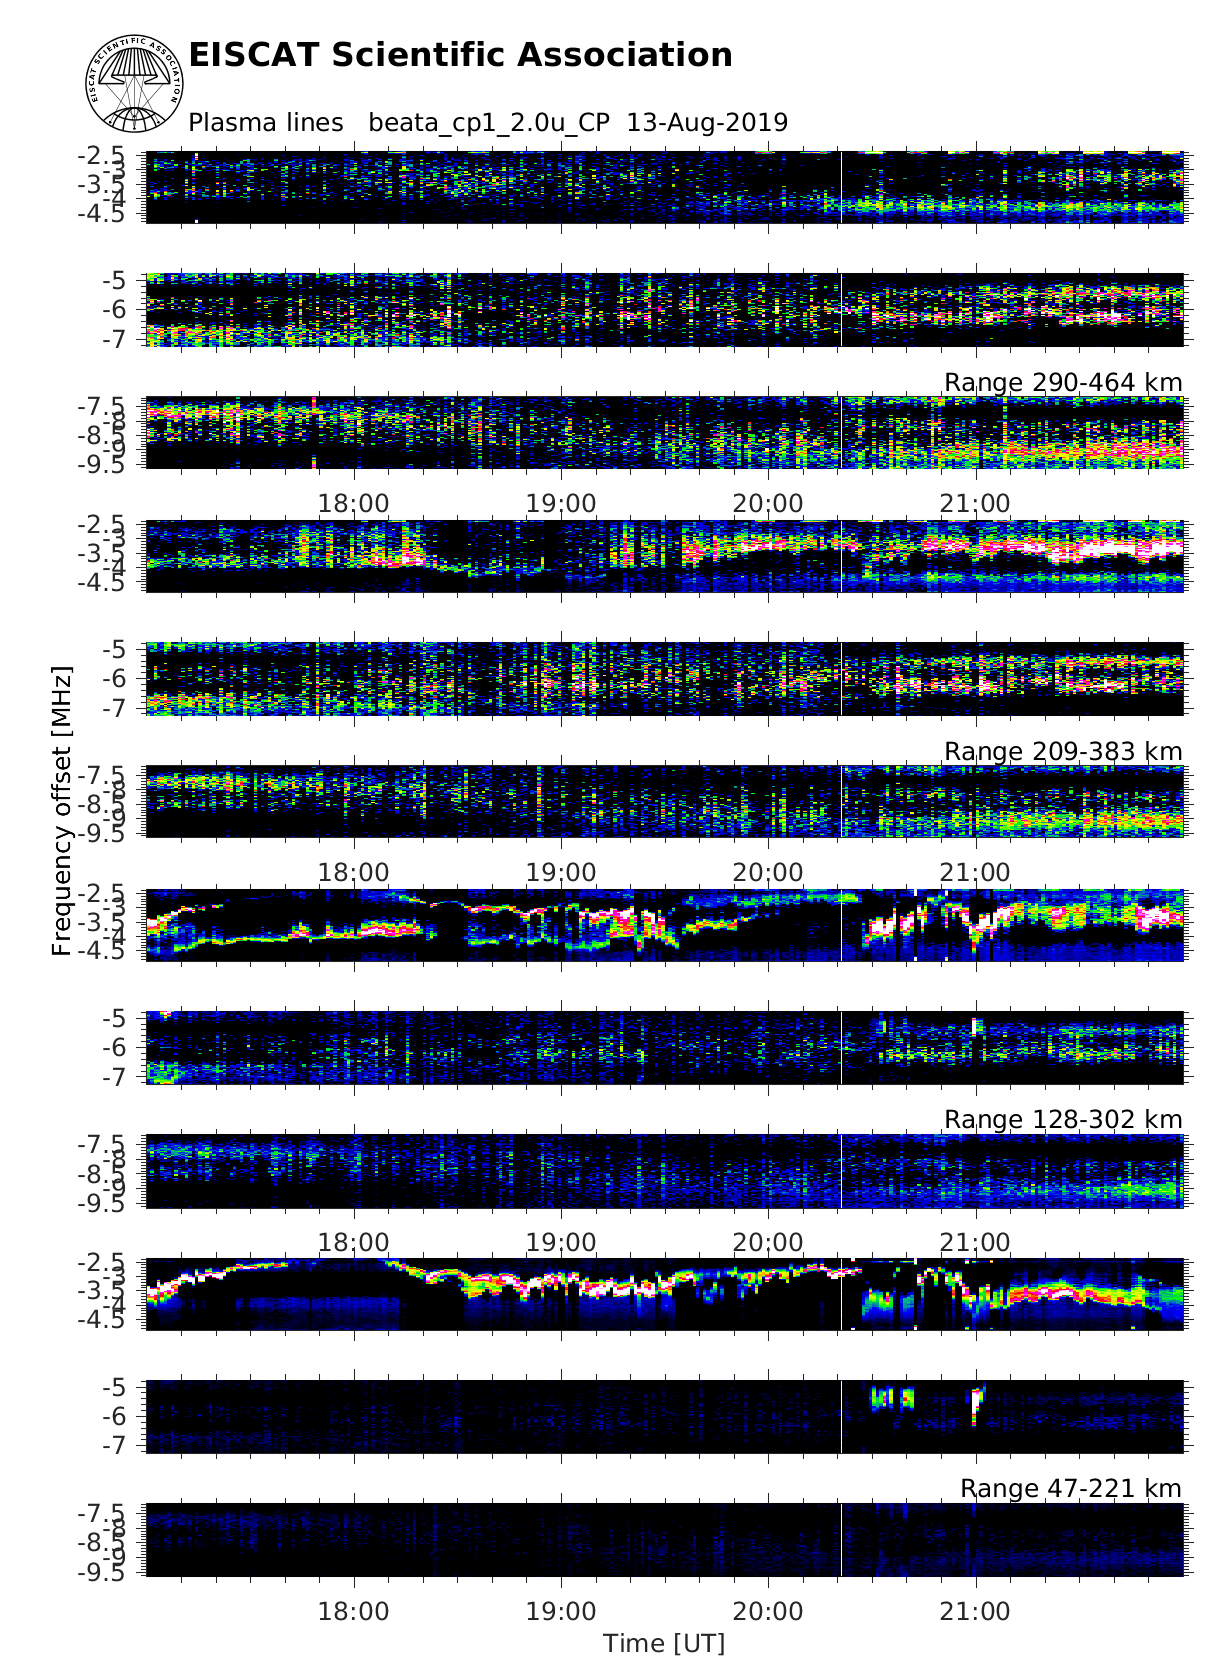
\includegraphics[width=\linewidth]{pl_spec}
  \end{center}
  \caption{\label{fig:pl-overview}The plasma line overview plot, here for \texttt{beata}. Spectrograms
    are shown for the three frequency regions of \texttt{beata} and four range
    intervals. Note that in this case, a radar school run of UHF cp1,
    we were lucky and saw strong enhanced plasma lines.}
\end{figure}

Next, the program will ask for start and stop times.  Look for time
intervals with clear plasma lines and restrict the start:stop time
interval accordingly.

The routine will then compare the identified plasma frequencies with
critical frequencies calculated from the electron density peaks and
fit a line through those points, excluding outliers (number of
standard deviations can be chosen when the program asks for
input).

The result for this particular example is shown in
Figure~\ref{fig:calib-pl-ne}. Note that the time interval
20:30---22:30 was selected because of the unambiguous strong plasma
lines seen in Figure~\ref{fig:pl-overview}. Other intervals contain
peaks that were misidentified.

The routine finally suggests a new calibration constant based on the
linear fit between detected plasma frequencies and those calculated
from ion line peak $N_\mathrm{e}$.

In this example the suggested calibration constant is
$\mathtt{Magic\_const}=0.6$. It can also be seen that the used
constant has the default value of $\mathtt{Magic\_const}=0.7$. In this
case the difference is not significant enough to warrant a reanalysis, but in case the plasma line calibration would give a significantly different result (which is not caused by any problems in the plasma line identification etc), then run the GUISDAP ion line analysis again with the new \texttt{Magic\_const} value.


\begin{figure}
  \begin{center}
    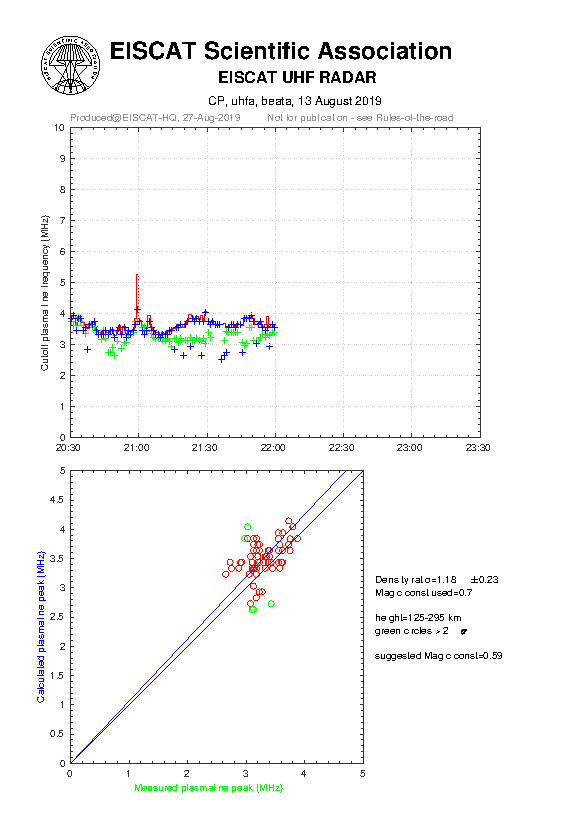
\includegraphics[width=0.9\linewidth]{2019-08-13_beata_60_pl_check_2030-2230@uhfa}
  \end{center}
  \caption{\label{fig:calib-pl-ne}Plasma line calibration. \newline
    Upper plot: ?? which colour is which data ?? \newline
    Lower plot: The identified plasma frequencies are compared with
    critical frequencies calculated from electron density peaks and a
    line is fitted. Green points indicate outliers that have been
    discarded (default outside $2\sigma{}$. A new calibration constant
    corresponding to the fitted line is suggested.}
  
\end{figure}


\clearpage{}

\section{Looking at plasma line spectra}
\label{sec:looking-at-plasma}

It may be useful to look visually for altitude-resolved plasma lines
in spectrograms, calculated by FFT on lag profile data. This is easy
by running GUISDAP with the following settings

\begin{description}
 
\item[Site] P
\item[Figures] 0 1 0 1 0
\item[Special] display\_spectra=1;
\end{description}

?? Check if both Site P and display\_spectra are necessary ??

With this selection, GUISDAP will not run the normal ion line
analysis, but show the plasma line spectra. They will look similar to
this figure (Figure~\ref{fig:pl-spec}).

\begin{figure}[b]
  \begin{center}
    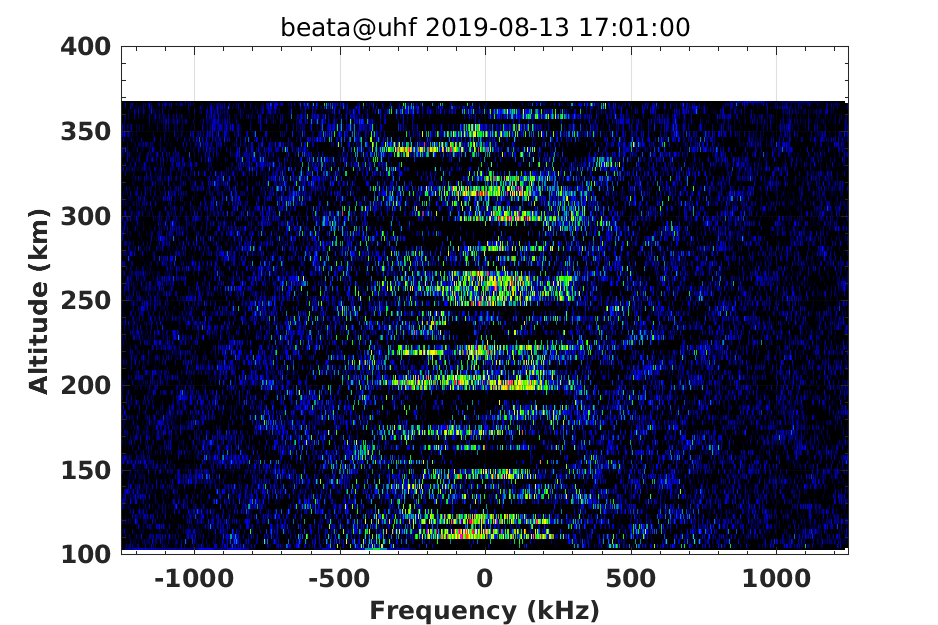
\includegraphics[width=0.8\linewidth]{pl_display_spec}
  \end{center}
  \caption{\label{fig:pl-spec}Running GUISDAP with site P (and/or Special argument \texttt{display\_spectra=1}) ?? Check which of these are necessary  ??. \newline{}Instead of the normal ion line analysis, figures similar to this one are shown.}
\end{figure}


Output files will still be saved. These will contain power profiles
and additional matrices containing the plasma line spectra
\begin{verbatim}
r_range
r_freq
r_spec
\end{verbatim}

Note however that the standard plasma line calibration routines expect
integrated data in the lag profile domain, not the spectra produced in
this way.



\end{document}

%%% Local Variables:
%%% mode: latex
%%% TeX-master: t
%%% End:
